\chapter{Theoretical framework}

\section{Phase-locked loop fundamentals}
\subsection{Basic concept}
The PLL is a feedback control system that is used to synchronize the phase and frequency of an output signal to a reference signal. The 
reference signal is a very stable clock signal locally generated usually by a crystal oscillator. The PLL compares the phase of this 
reference signal with the phase of the output signal and generates an error signal that is used to adjust the frequency of the output 
signal.

\noindent There's two types of applications for PLLs broadly speaking: clock generation and clock data recovery. In the first case,
the PLL is used to generate a clock signal that is synchronized to the reference signal. In the second case, the PLL is used to recover 
the clock signal from a data stream.

\noindent The PLL consists of three main components: a phase detector (PD), a loop filter (LF) and a voltage-controlled oscillator (VCO). 
The PD compares the phase of the reference signal with the phase of the output signal and generates an error signal that is proportional 
to the phase difference between the two signals. The LF smooths out the ripple riddled signal generated by the PD, reduces the high 
frequency noise of the loop and provides a stable control voltage to the VCO. The VCO generates an output signal whose frequency is 
proportional to the control voltage. Lastly, the output signal is fed back to the PD, thereby creating a closed-loop system.

\noindent If the PLL also has a frequency divider in the feedback path, the system is also capable of generating a frequency that is a
multiple or fraction of the reference frequency. This is useful in applications where a higher frequency is needed, 
such as in RF synthesizers.

\subsection{Key PLL parameters}
\subsubsection{Phase noise / jitter}
Jitter is defined as the time deviation ($\Delta_t$) of a signal's transition edges from their ideal positions in time. It is a metric of the outmost importance in the design of PLLs 
as it is a direct measure of the quality of the clock signal generated. Phase noise describes the same phenomenon in the frequency domain (the phase noise of a signal is the Fourier 
transform of the jitter) and is usually expressed in dBc/Hz.
\subsubsection{Output frequency}
It is defined as the range of frequencies that the PLL is capable of generating and can be determined by the VCO output range and the division ratio of the feedback frequency divider. This
is a key metric in establishing the application of the PLL (e.g., clock generation or RF synthesizer) and it bears significant importance in the design process due to the tradeoff 
it has with the phase noise performance of the PLL.
\subsubsection{Loop bandwidth}
The closed-loop bandwidth of a PLL is the frequency range over which the PLL can track the phase/frequency variations of the input signal 
(from DC to either -3 dB from the open-loop gain or to the unity-gain frequency at 0 dB). It affects the acquisition time and phase noise 
performance of the PLL.
\subsubsection{Noise bandwidth}
It is the PLL's noise due to the filter's loop bandwidth, the higher frequencies of the voltage-controlled oscillator (VCO) are the major
contributor to this effect, therefore the need to set a low enough bandwidth in order to suppress the most out of it. Even if reducing the loop
bandwidth would be desirable to suppress in-band phase noise, it's also necessary to take into consideration that there is a tradeoff between the
lock-in time and in-band phase noise.
\subsubsection{Beat-note period}
Defined as the time interval between successive "beats" (oscillations) observed at the phase detector output, in other words, is the inverse of
the frequency difference's magnitude between the reference and feedback signals as shown in figure \ref{fig:PFD_output}. Beat-note period is closely related to the acquisition time of the
PLL and can be estimated by equation \eqref{eq:T_beat}. This metric is a direct measure of the frequency mismatch between the reference and
the feedback signals.

\begin{equation}
    T_{beat} = \frac{1}{|f_{ref} - f_{feed}|}
    \label{eq:T_beat}
\end{equation}


\begin{minipage}{0.3\textwidth}
    \begin{center}
        \vspace{1.5 cm}
        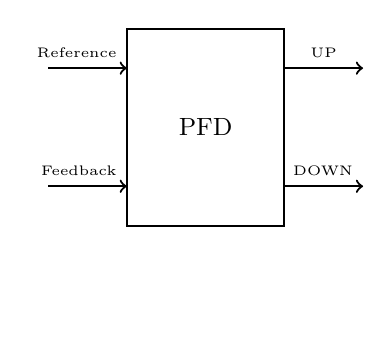
\begin{tikzpicture}
            \draw[white] (0,0) rectangle (2,-1.2);   %PFD
            \draw[->, thick] (-1,2) -- (0,2) node[anchor=south east] {\tiny Reference};
            \draw[->, thick] (-1, 0.5) -- (0,0.5) node[anchor=south east] {\tiny Feedback};
            \draw[thick] (0,0) rectangle (2,2.5);   %PFD
            \draw node at (1,1.25) {\small PFD};
            \draw[->, thick] (2,0.5) -- (3,0.5) node[anchor=south east] {\tiny DOWN};
            \draw[->, thick] (2,2) -- (3,2);
            \draw node at (2.5,2.2) {\tiny UP};
        \end{tikzpicture}
        \captionof{figure}{a) PFD block.}
        \label{fig:PFD_block}
    \end{center}
\end{minipage}
%\hspace{0.01\textwidth}
\begin{minipage}{0.7\textwidth}
    \begin{center}
        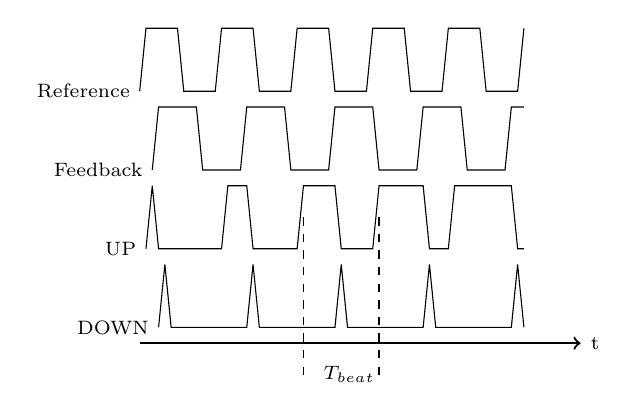
\begin{tikzpicture}[scale = 0.8]
            \draw[->, thick] (0,1) -- (7,1) node[anchor=west] {\scriptsize t};
            \draw (0,5) node[anchor=east] {\scriptsize Reference} -- (0.1,6) -- (0.6,6) -- (0.7,5) -- (1.2,5) -- (1.3,6) -- (1.8,6) -- (1.9,5) -- (2.4,5) -- (2.5,6) -- (3,6) -- (3.1,5) -- (3.6,5) -- (3.7,6) -- (4.2,6) -- (4.3,5) -- (4.8,5) -- (4.9,6) -- (5.4,6) -- (5.5,5) -- (6,5) -- (6.1,6);
            \draw (0.2,3.75) node[anchor=east] {\scriptsize Feedback} -- (0.3,4.75) -- (0.9,4.75) -- (1,3.75) -- (1.6,3.75) -- (1.7,4.75) -- (2.3,4.75) -- (2.4,3.75) -- (3,3.75) -- (3.1,4.75) -- (3.7,4.75) -- (3.8,3.75) -- (4.4,3.75) -- (4.5,4.75) -- (5.1,4.75) -- (5.2,3.75) -- (5.8,3.75) -- (5.9,4.75) -- (6.1,4.75);
            \draw (0.1,2.5) node[anchor=east] {\scriptsize UP} -- (0.2,3.5) -- (0.3,2.5) -- (1.3,2.5) -- (1.4,3.5) -- (1.7,3.5) -- (1.8,2.5) -- (2.5,2.5) -- (2.6,3.5) -- (3.1,3.5) -- (3.2,2.5) -- (3.7,2.5) -- (3.8,3.5) -- (4.5,3.5) -- (4.6,2.5) -- (4.9,2.5) -- (5,3.5) -- (5.9,3.5) -- (6,2.5) -- (6.1,2.5);
            \draw (0.3,1.25) node[anchor=east] {\scriptsize DOWN} -- (0.4,2.25) -- (0.5,1.25) -- (1.7,1.25) -- (1.8,2.25) -- (1.9,1.25) -- (3.1,1.25) -- (3.2,2.25) -- (3.3,1.25) -- (4.5,1.25) -- (4.6,2.25) -- (4.7,1.25) -- (5.9,1.25) -- (6,2.25) -- (6.1,1.25);
            \draw[dashed] (2.6,3) -- (2.6,0.5) node[right, outer sep=4pt] {\scriptsize $T_{beat}$};
            \draw[dashed] (3.8,3) -- (3.8,0.5);
        \end{tikzpicture}
        \captionof{figure}{b) PFD output.}
        \label{fig:PFD_output}
    \end{center}
\end{minipage}
\subsubsection{Lock-in time}
Lock-in time (also called aquisition or settling time) is defined as the time for the PLL to lock on to the input reference phase and frequency within one 
beat-note period ($T_{beat}$) after a frequency change or startup of the system. This parameter measures the time required for the PLL
to achieve the final phase lock once the VCO frequency is within the lock-in range. The lock-in time can be estimated with equation
\eqref{eq:lock-in_time}.

\begin{equation}
    T_{lock-in} = \frac{ln(\epsilon)}{\zeta \omega_{n}}
    \label{eq:lock-in_time}
\end{equation}

where:

\[\epsilon = \text{acceptable phase error}\]
\[\zeta = \text{damping factor}\]
\[\omega_{n} = \text{natural frequency}\]


\subsubsection{Pull-in time}
In contrast with the lock-in time, the pull-in time is the required amount of time for the PLL to initially aquire lock on to the 
reference signal from an arbitrary starting frequency (when the VCO's initial frequency is far from the target).
\subsubsection{Lock-in range}
The frequency range within which the PLL locks to the reference frequency in one $T_{beat}$. Once the feedback signal is in this 
range, the PLL will enter lock state within the next T$_{beat}$.
\subsubsection{Pull-in range}
Range of frequency within which the PLL can aquire lock on to the reference signal once the VCO has the correct frequency and several 
beat-note periods have passed.
\subsubsection{Pull-out range}
The maximum allowed frequency or phase abrupt change applied to the reference signal beyond which the PLL unlocks.
\subsubsection{Hold range}
This parameter establishes the maximun theoretical frequency range for an input reference beyond which the PLL never locks. Hold range
is bigger than both lock-in and pull-in ranges.
\subsubsection{SNR}
The signal to noise ratio is an appropiate way to measure the impact of noise on a circuit. It's often used in most figures
of merit (FOM) for making fair comparisons between PLLs.
\subsubsection{Power consumption}
An important parameter in measuring the performance of integrated circuits. Often used in most FOMs.
\subsubsection{Spurs}
Spurious tones are unwanted periodic signals that appear at the output spectrum of the PLL. Spurs are completely deterministic, thus they are distinct
from phase noise which is random and spreads across the spectrum of the signal.

\subsection{Analog phase-locked loop}
The principles of operation of the digital PLL stem from its analog counterpart, therefore this subsection describes the fundamental 
building blocks of the analog PLL as well as a simplified model of the system which allows for the circuit designer to analyze its behavior.

\subsubsection{Linear phase model of the PLL}
The PLL is a non-linear system, yet it can be approximated quite accurately into the linear system of figure \ref{fig:PFD_block} if certain
assumptions are taken in to consideration. The first of this assumptions is that the phase error ($\phi_{e}$) must be small enough, 
meaning the PLL is near lock state. Another one is that the characteristic of the phase detector must be approximately linear and given
by \eqref{eq:PD_linear_equation}. Lastly, the VCO's tuning range must be within its linear region of operation (it is generally desirable to limit the
variation of $K_{VCO}$ to no more than 20\%) like the frequency range between $\omega_1$ and $\omega_2$ in figure \ref{fig:VCO_characteristic_example}, only in this conditions the VCO can be considered
a linear system and thus be described by \eqref{eq:VCO_linear_equation}.  

\begin{center}
        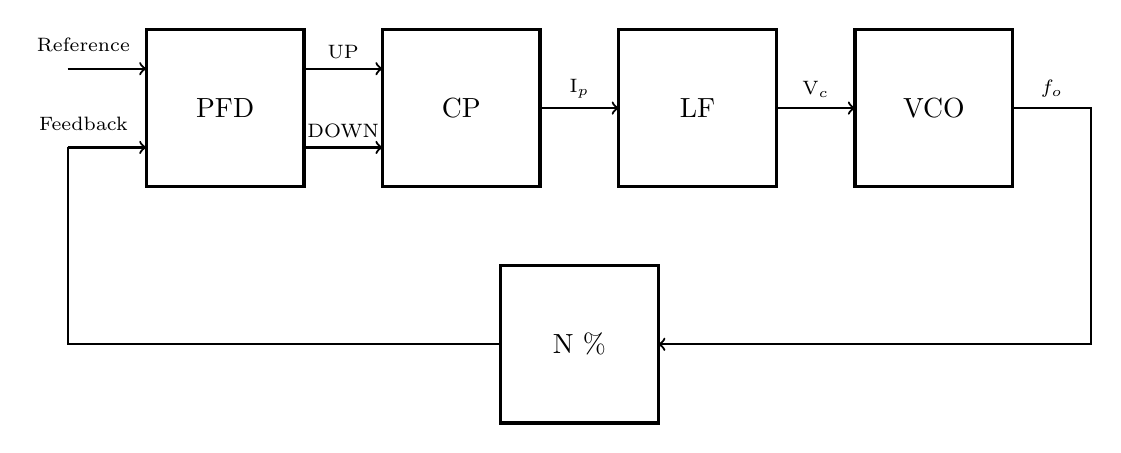
\begin{tikzpicture}
            [
                block/.style={rectangle, very thick, draw=black, minimum size=5pt}
            ]
            % PFD
            \draw[very thick] (0,3) rectangle (2,5);
            \draw node at (1,4) {PFD};
            \draw[->, thick] (2,4.5) -- node[above] {\scriptsize UP} (3,4.5);
            \draw[->, thick] (2,3.5) -- node[above] {\scriptsize DOWN} (3, 3.5);
            \draw[->, thick] (-1,4.5) -- (0,4.5);
            \draw[->, thick] (-1,3.5) -- (0, 3.5);
            \draw node at (-0.8,4.8) {\scriptsize Reference};
            \draw node at (-0.8,3.8) {\scriptsize Feedback};
            % CP
            \draw[very thick] (3,3) rectangle (5,5);
            \draw node at (4,4) {CP};
            \draw[->, thick] (5,4) -- node[above] {\scriptsize I$_{p}$} (6,4);
            % LF
            \draw[very thick] (6,3) rectangle (8,5);
            \draw node at (7,4) {LF};
            \draw[->, thick] (8,4) -- node[above] {\scriptsize V$_{c}$} (9,4);
            % VCO
            \draw[very thick] (9,3) rectangle (11,5);
            \draw node at (10,4) {VCO};
            \draw[->, thick] (11,4) -- node[above] {\scriptsize $f_{o}$} (12,4) -- (12,1) -- (6.5,1);
            % N %
            \draw[very thick] (4.5,0) rectangle (6.5,2);
            \draw node at (5.5,1) {N \%};
            \draw[thick] (4.5,1) -- (-1,1) -- (-1,3.5);
        \end{tikzpicture}
        \captionof{figure}{Block diagram of the linear phase PLL.}
        \label{fig:PLL_block_diagram}
\end{center}

\begin{equation}
    v_{d} = K_{PD} \, \phi{e} + \underbrace{V_{do}}_{\text{\tiny free running voltage}}
    \label{eq:PD_linear_equation}
\end{equation}
\begin{equation}
    \Delta_{\omega_{o}} = K_{VCO} \, (V_{c} - V_{co})
    \label{eq:VCO_linear_equation}
\end{equation}

\noindent Each of the blocks in \ref{fig:PLL_block_diagram} has a transfer function associated with it, which can be expressed as follows:
The PFD/CP combination is modeled as a current source with a gain of $I_{p}/2\pi$. The VCO is modeled as an ideal integrator with gain 
$K_{VCO}$ and its transfer function is given by $K_{VCO}/S$. The feedback divider is modeled as a simple gain of $1/N$. Finally, the loop
filter (LF) depends on the order of the filter and the type of components used. 

\begin{minipage}{0.45\textwidth}
    \begin{center}
        \begin{tikzpicture}
            \begin{axis}[
                axis lines=left,
                width=\textwidth,
                %height=0.25\textwidth,
                xlabel={\scriptsize V$_{control}$ [V]},
                ylabel={\scriptsize $\Delta_{\omega_{o}}$ [rad/s]},
                xtick={0.1, 0.62},
                ytick={1.001000000, 1.007000000},
                xticklabels={$V_1$, $V_2$},
                grid=major,
                yticklabels={$\omega_1$, $\omega_2$}
            ]
                \addplot[
                    mark size=0.5pt,  % Setting mark size
                ]
                table[meta=freq]
                {data/VCO_characteristic_example.txt};   % Reading data from dataFile.txt
            \end{axis}
        \end{tikzpicture}
        \captionof{figure}{VCO characteristic example.}
        \label{fig:VCO_characteristic_example}
    \end{center}
\end{minipage}
\hspace{0.01\textwidth}
\begin{minipage}{0.45\textwidth}
    \begin{center}
        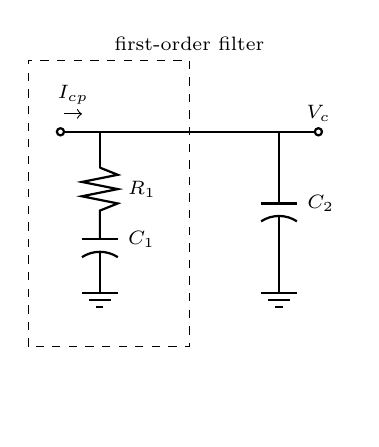
\begin{tikzpicture}[scale=0.91]
            \draw[color=white] (-3.5,-4) rectangle (1,-3);
            \draw[dashed] (-3.5,-3) rectangle (-1.25,1) node[above] {\scriptsize first-order filter};
            \draw[thick] (-3.05,0) circle (0.05);
            \draw[thick] (0.55,0) circle (0.05) node[above] {\scriptsize $V_{c}$};
            \draw[thick] (-3,0) -- (0.5,0);
            \draw[->] (-3,0.25) -- node[above]{\scriptsize $I_{cp}$} (-2.75,0.25);
            \draw[thick] (-2.5,0) -- (-2.5,-0.5);
            \draw[thick] (-2.5,-0.5) -- (-2.25,-0.6) -- (-2.75,-0.7) -- (-2.25,-0.8) node[right] {\scriptsize $R_1$} -- (-2.75,-0.9) -- (-2.25,-1) -- (-2.5,-1.1) -- (-2.5,-1.5);
            \draw[thick] (-2.75,-1.5) -- (-2.25,-1.5) node[right] {\scriptsize $C_1$};
            \draw[thick] (-2.75,-1.75) .. controls (-2.6,-1.65) and (-2.4,-1.65) .. (-2.25,-1.75);
            \draw[thick] (-2.5,-1.675) -- (-2.5,-2.25);
            \draw[thick] (-2.75,-2.25) -- (-2.25,-2.25);
            \draw[thick] (-2.65,-2.35) -- (-2.35,-2.35);
            \draw[thick] (-2.55,-2.45) -- (-2.45,-2.45);
            \draw[thick] (0,0) -- (0,-1);
            \draw[thick] (-0.25,-1) -- (0.25,-1) node[right] {\scriptsize $C_2$};
            \draw[thick] (-0.25,-1.25) .. controls (-0.1,-1.15) and (0.1,-1.15) .. (0.25,-1.25);
            \draw[thick] (0,-1.175) -- (0,-2.25);
            \draw[thick] (-0.25,-2.25) -- (0.25,-2.25);
            \draw[thick] (-0.15,-2.35) -- (0.15,-2.35);
            \draw[thick] (-0.05,-2.45) -- (0.05,-2.45);
        \end{tikzpicture}
        \captionof{figure}{Second-order passive loop filter.}
        \label{fig:LF_schematic}
    \end{center}
\end{minipage}

\noindent The most common implementation is a passive RC filter, which can be modeled either as a first-order or a second-order system. 
For the sake of simplicity in this analysis, the LF is modeled as a first-order circuit like the one enclosed by dashed lines in figure 
\ref{fig:LF_schematic}. The transfer function of the LF is then given by $(R_1 S C_1 + 1) / (S C_1)$.

\noindent Knowing the transfer functions of each block, one can represent the PLL system as in figure \ref{fig:PLL_block_diagram_TF}.
Then with the help of Mason's rule \eqref{eq:Masons_rule}, the overall closed-loop transfer function \eqref{eq:ACL} of the PLL can be obtained.

\begin{equation}
    H(s) = \frac{\Sigma_{F.P} (1 - \Sigma_{loops \, not \, touching})}{1 - \Sigma_{loops}}
    \label{eq:Masons_rule}
\end{equation}

\begin{center}
    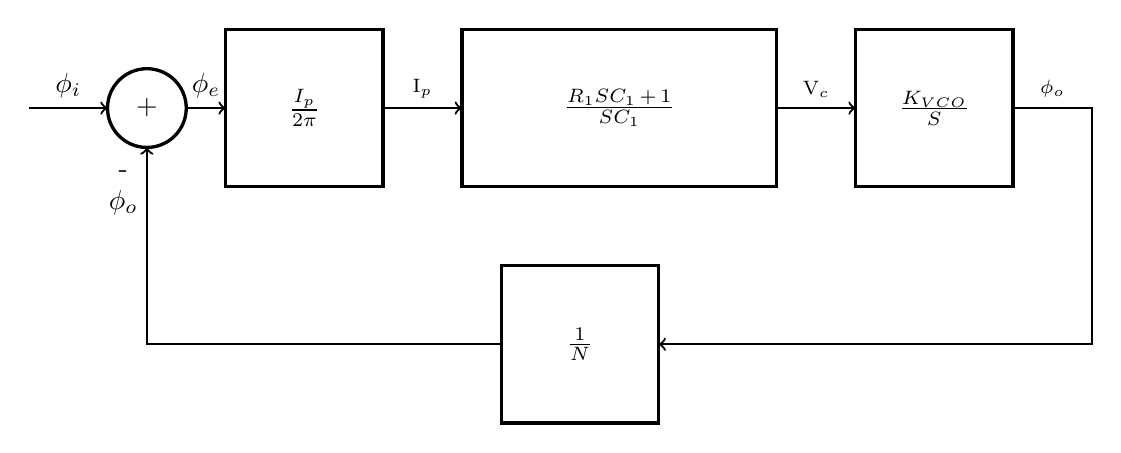
\begin{tikzpicture}
        [
            block/.style={rectangle, very thick, draw=black, minimum size=5pt}
        ]
        % PFD
        \draw[very thick] (0,4) circle (0.5);
        \draw node at (0,4) {+};
        \draw[->, thick] (0.5,4) -- node[above] {$\phi_{e}$} (1,4);
        \draw[->, thick] (-1.5,4) -- node[above] {$\phi_{i}$} (-0.5,4);
        \draw node at (-0.3,2.8) {$\phi_{o}$};
        \draw node at (-0.3,3.2) {-};
        % CP
        \draw[very thick] (1,3) rectangle (3,5);
        \draw node at (2,4) {$\frac{I_{p}}{2\pi}$};
        \draw[->, thick] (3,4) -- node[above] {\scriptsize I$_{p}$} (4,4);
        % LF
        \draw[very thick] (4,3) rectangle (8,5);
        \draw node at (6,4) {$\frac{R_1 S C_{1} \, + \, 1}{S C_1}$};
        \draw[->, thick] (8,4) -- node[above] {\scriptsize V$_{c}$} (9,4);
        % VCO
        \draw[very thick] (9,3) rectangle (11,5);
        \draw node at (10,4) {$\frac{K_{VCO}}{S}$};
        \draw[->, thick] (11,4) -- node[above] {\scriptsize $\phi_{o}$} (12,4) -- (12,1) -- (6.5,1);
        % N %
        \draw[very thick] (4.5,0) rectangle (6.5,2);
        \draw node at (5.5,1) {$\frac{1}{N}$};
        \draw[->, thick] (4.5,1) -- (0,1) -- (0,3.5);
    \end{tikzpicture}
    \captionof{figure}{Block diagram of the linear phase PLL with each block transfer function.}
    \label{fig:PLL_block_diagram_TF}
\end{center}

\begin{equation}
    A_{CL} = \frac{\frac{I_p K_{VCO}}{2 \pi C_1} (R_1 S C_1 \, + \, 1)}{S^2 \, + \, S \frac{I_p}{2 \pi} K_{VCO} R_1 \, + \, \frac{I_p K_{VCO}}{2 \pi C_1}}
    \label{eq:ACL}
\end{equation}

\noindent From the closed-loop transfer function \eqref{eq:ACL} one can see that the PLL behaves as a second-order system with two poles at the 
origin (two ideal integrators), opening up the possibility of instability. In order to ensure stability, the PLL must be designed to have 
a sufficiently high phase margin ($\phi_m$), and consequently an adequate damping factor ($\zeta$) and natural frequency ($\omega_{n}$). 
Both $\omega_{n}$ \eqref{eq:omega_n} and $\zeta$ \eqref{eq:zeta} are crucial parameters in the design of the PLL, as they determine the bandwidth
and transient response of the system.

\begin{equation}
    \omega_{n} = \sqrt{\frac{I_p K_{VCO}}{2 \pi C_1}}
    \label{eq:omega_n}
\end{equation}
\begin{equation}
    \zeta = \frac{R_1}{2} \sqrt{\frac{I_p K_{VCO} C_1}{2 \pi}}
    \label{eq:zeta}
\end{equation}

\noindent It can be proven that the loop bandwidth ($\omega_u$) is related with $\omega_{n}$ and $\zeta$ by equation \eqref{eq:loop_bandwidth}.

\begin{equation}
    \omega_{u}^2 = (2 \zeta^2 \, + \, \sqrt{4 \zeta^4 \, + \, 1}) \omega_{n}^2
    \label{eq:loop_bandwidth}
\end{equation}

\subsubsection{Phase frequency detector}

A PLL that has a phase frequency detector (PFD) instead of just a phase detector (PD) is superior because it can track changes in both
phase and frequency at the input signal. This approach provides robustness to the system because the PLL locks regardless of the initial
value of the output frequency, therefore making the pull-in range equal to the VCO tuning range.

\noindent The most common implementation of a PFD is shown in figure \ref{fig;PFD_schematic}. The operation of this circuit is as follows:
When either of the two signals arrive with a rising edge to the corresponding D flip-flop CLK terminal a HIGH state is pass along
to its output (Q), this result is maintained until the other signal's rising edge arrives at the second flip-flop because at that
moment in time the AND gate would activate and reset both flip-flops. This behavior can be observed in figure \ref{fig:PFD_transient_response}.

\begin{minipage}{0.45\textwidth}
    \begin{center}
        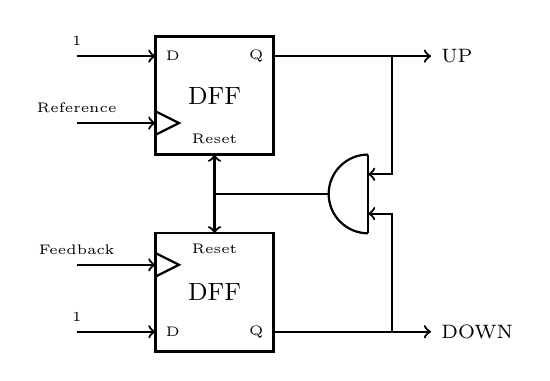
\begin{tikzpicture}[]
            \draw[thick] (0,0) rectangle (1.5,1.5);
            \draw[thick] (0,0.25) -- (0,0.55) -- (0.3,0.4) -- (0,0.25);
            \draw[->, thick] (-1,0.4) node[anchor=south] {\tiny Reference} -- (0,0.4);
            \draw node at (0.75,0.75) {\small DFF};
            \draw[->, thick] (-1,1.25) node[anchor=south] {\tiny 1} -- (0,1.25) node[anchor=west] {\tiny D};
            \draw[->, thick] (1.5,1.25) node[anchor=east] {\tiny Q} -- (3.5,1.25) node[right] {\scriptsize UP};
            \draw node at (0.75, 0.2) {\tiny Reset};
            
            \draw[thick] (0,-1) rectangle (1.5,-2.5);
            \draw[thick] (0,-1.25) -- (0,-1.55) -- (0.3,-1.4) -- (0,-1.25);
            \draw[->, thick] (-1,-1.4) node[anchor=south] {\tiny Feedback} -- (0,-1.4);
            \draw node at (0.75,-1.75) {\small DFF};
            \draw[->, thick] (-1,-2.25) node[anchor=south] {\tiny 1} -- (0,-2.25) node[anchor=west] {\tiny D};
            \draw[->, thick] (1.5,-2.25) node[anchor=east] {\tiny Q} -- (3.5,-2.25) node[anchor=west] {\scriptsize DOWN};
            \draw node at (0.75, -1.2) {\tiny Reset};
    
            \draw[->, thick] (3,1.25) -- (3,-0.25) -- (2.7,-0.25);
            \draw[->, thick] (3,-2.25) -- (3,-0.75) -- (2.7,-0.75);
            \draw[thick] (2.7,0) -- (2.7,-1);
            \draw[thick] (2.7,0) arc (90:270:0.5);
            \draw[->, thick] (2.2,-0.5) -- (0.75,-0.5) -- (0.75,0);
            \draw[->, thick] (0.75,-0.5) -- (0.75,-1);

            %\draw[red] (0,-2.5) rectangle (1.5,-4);
        \end{tikzpicture}
        \captionof{figure}{Three states PFD implementation.}
        \label{fig;PFD_schematic}
    \end{center}
\end{minipage}
\hspace{0.01\textwidth}
\begin{minipage}{0.45\textwidth}
    \begin{center}
        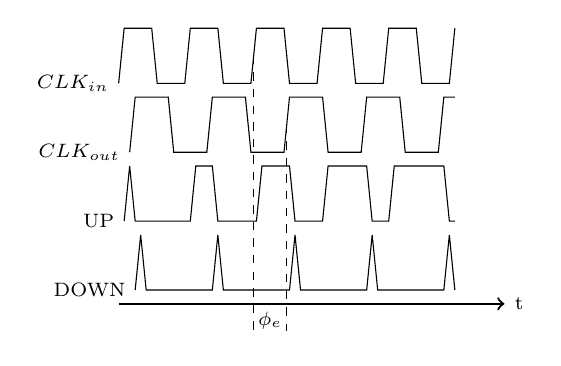
\begin{tikzpicture}[scale=0.7]
            \draw[->, thick] (0,1) -- (7,1) node[anchor=west] {\scriptsize t};
            \draw (0,5) node[anchor=east] {\scriptsize $CLK_{in}$} -- (0.1,6) -- (0.6,6) -- (0.7,5) -- (1.2,5) -- (1.3,6) -- (1.8,6) -- (1.9,5) -- (2.4,5) -- (2.5,6) -- (3,6) -- (3.1,5) -- (3.6,5) -- (3.7,6) -- (4.2,6) -- (4.3,5) -- (4.8,5) -- (4.9,6) -- (5.4,6) -- (5.5,5) -- (6,5) -- (6.1,6);
            \draw (0.2,3.75) node[anchor=east] {\scriptsize $CLK_{out}$} -- (0.3,4.75) -- (0.9,4.75) -- (1,3.75) -- (1.6,3.75) -- (1.7,4.75) -- (2.3,4.75) -- (2.4,3.75) -- (3,3.75) -- (3.1,4.75) -- (3.7,4.75) -- (3.8,3.75) -- (4.4,3.75) -- (4.5,4.75) -- (5.1,4.75) -- (5.2,3.75) -- (5.8,3.75) -- (5.9,4.75) -- (6.1,4.75);
            \draw (0.1,2.5) node[anchor=east] {\scriptsize UP} -- (0.2,3.5) -- (0.3,2.5) -- (1.3,2.5) -- (1.4,3.5) -- (1.7,3.5) -- (1.8,2.5) -- (2.5,2.5) -- (2.6,3.5) -- (3.1,3.5) -- (3.2,2.5) -- (3.7,2.5) -- (3.8,3.5) -- (4.5,3.5) -- (4.6,2.5) -- (4.9,2.5) -- (5,3.5) -- (5.9,3.5) -- (6,2.5) -- (6.1,2.5);
            \draw (0.3,1.25) node[anchor=east] {\scriptsize DOWN} -- (0.4,2.25) -- (0.5,1.25) -- (1.7,1.25) -- (1.8,2.25) -- (1.9,1.25) -- (3.1,1.25) -- (3.2,2.25) -- (3.3,1.25) -- (4.5,1.25) -- (4.6,2.25) -- (4.7,1.25) -- (5.9,1.25) -- (6,2.25) -- (6.1,1.25);
            \draw[dashed] (2.45,5.5) -- (2.45,0.5);
            \draw node at (2.75,0.7) {\scriptsize $\phi_{e}$};
            \draw[dashed] (3.05,4.25) -- (3.05,0.5);
        \end{tikzpicture}
        \captionof{figure}{Transient response of the PFD.}
        \label{fig:PFD_transient_response}
    \end{center}
\end{minipage}

\subsubsection{Loop filter}
The function of the loop filter is to filter out the high frequency noise from the VCO and to provide a stable control voltage to the VCO.
The loop filter is usually a passive RC filter as the one in figure \ref{fig:LF_schematic}, but it can also be an active filter. The loop 
filter is a critical component of the PLL because it determines the bandwidth, the noise performance and the transient response of the PLL.
The loop filter is usually designed to be a second-order low-pass filter, but it can also be a higher-order filter if needed. The values 
of the components of the filter should be designed first and foremost to achieve stability at a given bandwidth, equations
\eqref{eq:zeta} and \eqref{eq:loop_bandwidth} are useful for this purpose.

\noindent The -3dB closed-loop bandwidth and the open-loop unity-gain bandwidth are fairly close to each other for $\zeta \geq 1$. It is 
for this reason that both quantities are often used interchangeably. In order to achieve a good transient response and noise performance,
the loop bandwidth should be set to a value of $\omega_{ref}/10 \, [rad/s]$ or less, where $\omega_{ref}$ is the reference frequency.
\subsubsection{Charge pump}
Charge pumps (CP) are circuits designed to either source or sink charge to/from a capacitor for a controlled amount of time. There are
many different implementations of charge pumps, but all of them consist of a current source, a switch and a capacitor (which is usually 
part of the loop filter). Most of the PLLs designed today are CPPLLs (or type-II PLLs) because the combination of PFD/CP/LF exhibit an 
infinite gain for a finite phase error, which means that for the control voltage to be finite, the phase error must be zero. This is a 
desirable property because it allows the PLL to have a very low phase error. Figure \ref{fig:CP_diagram} shows the diagram of a
charge pump, while figure \ref{fig:CP_schematic} shows the schematic of a CMOS drain switched charge pump.
\begin{minipage}{0.49\textwidth}
    \begin{center}
        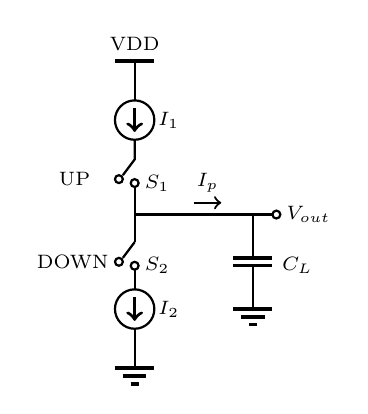
\begin{tikzpicture}
            \draw[very thick] (0,0) -- node[above]{\scriptsize VDD} (0.5,0);
            \draw[thick] (0.25,0) -- (0.25,-0.5);
            \draw[thick] (0.25,-0.75) circle (0.25);
            \draw[very thick, ->] (0.25,-0.6) -- node[inner sep = 8, right] {\scriptsize $I_1$} (0.25,-0.9);
            \draw[thick] (0.25,-1) -- (0.25,-1.25) -- (0.1,-1.45);
            \draw[thick] (0.05,-1.5) circle (0.05) node[inner sep = 10, left] {\scriptsize UP};
            \draw[thick] (0.25,-1.6) -- (0.25,-2.3);
            \draw[thick] (0.25,-1.55) circle (0.05) node[right] {\scriptsize $S_1$};
            \draw[thick] (0.25,-2.3) -- (0.1,-2.5);
            \draw[thick] (0.05,-2.55) circle (0.05) node[left] {\scriptsize DOWN};
            \draw[thick] (0.25,-2.65) -- (0.25,-2.9);
            \draw[thick] (0.25,-2.6) circle (0.05) node[right] {\scriptsize $S_2$};
            \draw[thick] (0.25,-3.15) circle (0.25);
            \draw[very thick, ->] (0.25,-3) -- node[inner sep = 8, right] {\scriptsize $I_2$} (0.25,-3.3);
            \draw[thick] (0.25,-3.4) -- (0.25,-3.9);
            \draw[very thick] (0,-3.9) -- (0.5,-3.9);
            \draw[very thick] (0.1,-4) -- (0.4,-4);
            \draw[very thick] (0.2,-4.1) -- (0.3,-4.1);

            \draw[thick] (0.25,-1.95) -- (2,-1.95);
            \draw[thick, ->] (1,-1.8) -- node[above]{\scriptsize $I_p$} (1.35,-1.8); 
            \draw[thick] (2.05,-1.95) circle (0.05) node[right] {\scriptsize $V_{out}$};
            \draw[thick] (1.75,-1.95) -- (1.75,-2.5);
            \draw[very thick] (1.5,-2.5) -- (2,-2.5);
            \draw[very thick] (1.5,-2.6) -- node[inner sep = 10, right]{\scriptsize $C_L$} (2,-2.6);
            \draw[thick] (1.75,-2.6) -- (1.75,-3.15);
            \draw[very thick] (1.5,-3.15) -- (2,-3.15);
            \draw[very thick] (1.6,-3.25) -- (1.9,-3.25);
            \draw[very thick] (1.7,-3.35) -- (1.8,-3.35);
        \end{tikzpicture}
        \captionof{figure}{Charge pump schematic.}
        \label{fig:CP_diagram}
    \end{center}
\end{minipage}
%\hspace{0.01\textwidth}
\begin{minipage}{0.49\textwidth}
    \begin{center}
        \vspace{4 mm}
        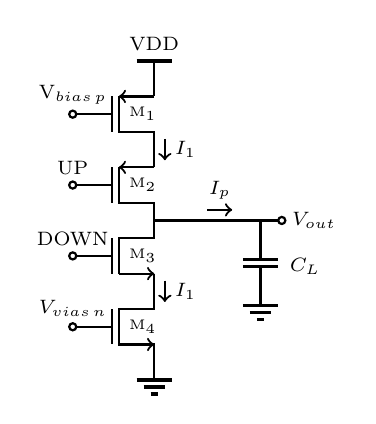
\begin{tikzpicture}[scale = 0.9]
            \draw[very thick] (0,0) -- node[above]{\scriptsize VDD} (0.5,0);
            \draw[thick] (0.25,0) -- (0.25,-0.5);
            \draw[thick, ->] (0.25,-0.5) -- (-0.25,-0.5);
            \draw[thick] (-0.25,-0.5) -- node[right]{\tiny M$_1$} (-0.25,-1) -- (0.25,-1) -- (0.25,-1.5);
            \draw[thick, ->] (0.25,-1.5) -- (-0.25,-1.5);
            \draw[thick] (-0.25,-1.5) -- node[right]{\tiny M$_2$} (-0.25,-2) -- (0.25,-2) -- (0.25,-2.5) -- (-0.25,-2.5) -- node[right]{\tiny M$_3$} (-0.25,-3);
            \draw[thick, ->] (-0.25,-3) -- (0.25,-3);
            \draw[thick] (0.25,-3) -- (0.25,-3.5) -- (-0.25,-3.5) -- node[right]{\tiny M$_4$} (-0.25,-4) -- (0.25,-4) -- (0.25,-4.5);
            \draw[thick, ->] (-0.25,-4) -- (0.25,-4);
            \draw[very thick] (0,-4.5) -- (0.5,-4.5);
            \draw[very thick] (0.1,-4.6) -- (0.4,-4.6);
            \draw[very thick] (0.2,-4.7) -- (0.3,-4.7);
            
            \draw[thick, ->] (0.4,-1.1) -- node[right]{\scriptsize $I_1$} (0.4,-1.4);
            \draw[thick, ->] (0.4,-3.1) -- node[right]{\scriptsize $I_1$} (0.4,-3.4);
            \draw[thick] (-0.35,-0.5) -- (-0.35,-1);
            \draw[thick] (-0.35,-1.5) -- (-0.35,-2);
            \draw[thick] (-0.35,-2.5) -- (-0.35,-3);
            \draw[thick] (-0.35,-3.5) -- (-0.35,-4);
            \draw[thick] (-0.35,-0.75) -- (-0.85,-0.75);
            \draw[thick] (-0.35,-1.75) -- (-0.85,-1.75);
            \draw[thick] (-0.35,-2.75) -- (-0.85,-2.75);
            \draw[thick] (-0.35,-3.75) -- (-0.85,-3.75);
            \draw[thick] (-0.9,-0.75) circle (0.05) node[above] {\scriptsize V$_{bias \, p}$};
            \draw[thick] (-0.9,-1.75) circle (0.05) node[above] {\scriptsize UP};
            \draw[thick] (-0.9,-2.75) circle (0.05) node[above] {\scriptsize DOWN};
            \draw[thick] (-0.9,-3.75) circle (0.05) node[above] {\scriptsize $V_{vias \, n}$};

            \draw[thick] (0.25,-2.25) -- (2,-2.25);
            \draw[thick, ->] (1,-2.1) -- node[above]{\scriptsize $I_p$} (1.35,-2.1); 
            \draw[thick] (2.05,-2.25) circle (0.05) node[right] {\scriptsize $V_{out}$};
            \draw[thick] (1.75,-2.25) -- (1.75,-2.8);
            \draw[very thick] (1.5,-2.8) -- (2,-2.8);
            \draw[very thick] (1.5,-2.9) -- node[inner sep = 10, right]{\scriptsize $C_L$} (2,-2.9);
            \draw[thick] (1.75,-2.9) -- (1.75,-3.45);
            \draw[very thick] (1.5,-3.45) -- (2,-3.45);
            \draw[very thick] (1.6,-3.55) -- (1.9,-3.55);
            \draw[very thick] (1.7,-3.65) -- (1.8,-3.65);
        \end{tikzpicture}
        \captionof{figure}{CMOS drain switched charge pump.}
        \label{fig:CP_schematic}
    \end{center}
\end{minipage}

\noindent The greatest challenge in designing a charge pump resides in eliminating any current mismatch between $I_1$ and $I_2$ while maintaining a
large output voltage compliance. This task is particularly difficult to achieve because the channel length modulation in the MOSFETs
causes the output current to be dependent on the output voltage ($V_{DS}$ modulates the current). This means that both the output voltage
compliance and the current mismatch performance trade off with each other.

The current mismatch ($I_{up} - I_{down}$) flows through the loop filter for the time it takes the PFD to reset both the UP and DOWN signals (approximately 5 gate delays) in every
input period. The cumulative effect implies that $V_{control} \to \infty $, which cannot happen because the PLL attempts to lock and keep the output frequency constant
\cite{bib:Razavi_PLL_book}. consequently, the loop will settle with a steady-state phase error ($\Delta_t$) and thus, the smaller current will last longer to keep the charge
constant. This behavior of the CP is illustrated in figure \ref{fig:CP_transient_response}.

\noindent The static phase error $\Delta_t$ can be approximated by equation \eqref{eq:steady_state_phase_error} in the steady state because the rise and fall of $V_{cntrl}$ must cancel each 
other out. The peak-to-peak amplitude ripple in $V_{cntrl}$ on the other hand can be estimated with equation \eqref{eq:V_control_ripple}.

\pagebreak

\begin{equation}
    \Delta_t = \frac{I_{up} - I_{down}}{I_{p}} \cdot t_{res}
    \label{eq:steady_state_phase_error}
\end{equation}

\noindent Where $t_{res}$ is the time it takes the PFD to reset both the UP and DOWN signals, and $I_{p}$ is the nominal charge pump current.

\begin{equation}
    \Delta V_{cntrl} = \frac{I_{up} - I_{down}}{C_L} \cdot t_{res}
    \label{eq:V_control_ripple}
\end{equation}

\begin{figure}[H]
    \centering
    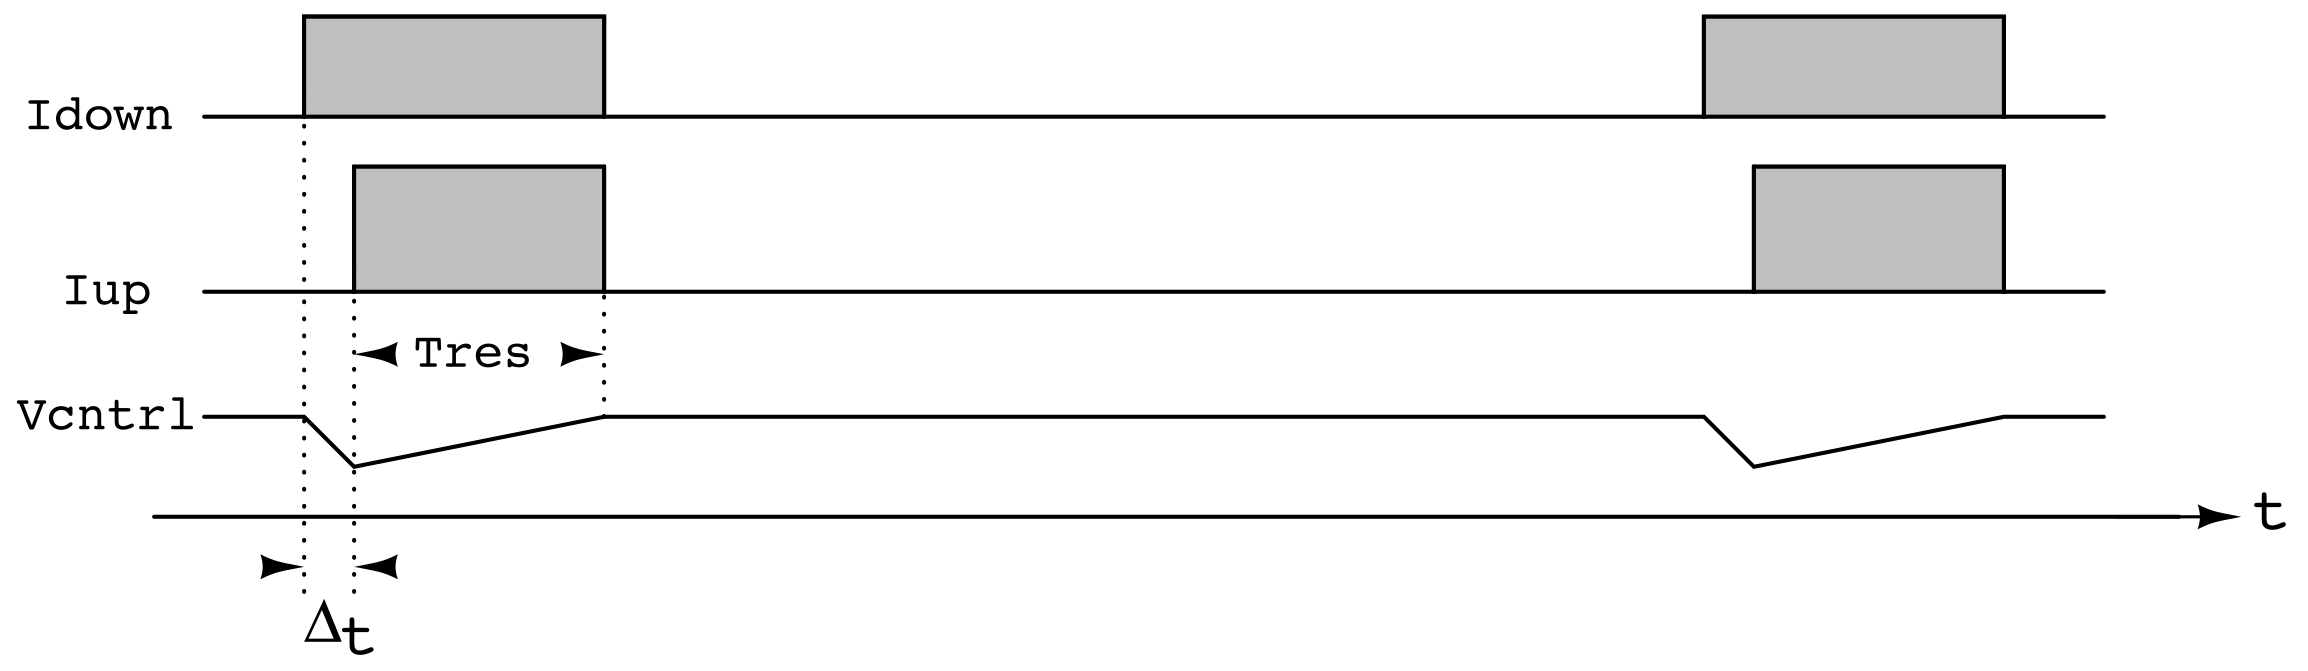
\includegraphics[width=1\textwidth]{figures/CP_transient_response.png}
    \caption{Charge pump transient response due to current mismatch.}
    \label{fig:CP_transient_response}
\end{figure}

\noindent There are multiple approaches to minimize this problem (some involving more complex topologies dealing also with the issue of clock feedthrough), yet 
the simplest one is to use wide enough (also large enough in the case of the current sources) transistors to minimize the channel length 
modulation effect. This solution is far from ideal, but is good enough for some applications.

\subsubsection{Voltage-controlled oscillator}
The VCO is the block that generates the output signal of the PLL. The frequency of the output signal is determined by the control voltage
that the loop filter provides. It is a non-linear circuit that converts a voltage into a frequency (though it can be assumed to be linear 
for the conditions mentioned in the previous section). The VCO response looks like that of figure \ref{fig:VCO_response}, where the gain 
of the VCO ($K_{VCO}$) is an important design parameter. In general, it is desirable to have a relatively small (without compromising the 
stability of the PLL) $K_{VCO}$ value so that any noise coupled to the previous stage does not translate into a large phase/frequency 
fluctuation at the output. A good rule of thumb is to keep $K_{VCO}$ below $0.1 f_m Hz/V$ where $f_m$ is the center frequency of the VCO
tuning range.

\begin{minipage}{0.4\textwidth}
    \begin{center}
        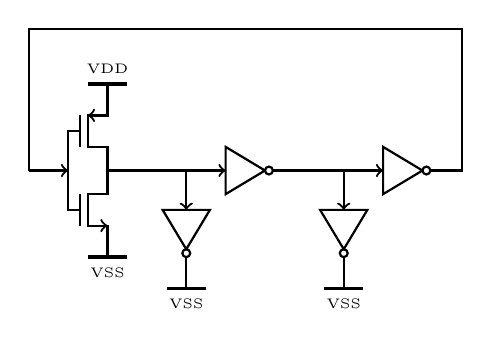
\begin{tikzpicture}
            \draw[thick, ->] (0,0) -- (0.5,0);
            \draw[very thick] (0.75,1.1) -- node[above]{\tiny VDD} (1.25,1.1);
            \draw[very thick] (0.75,-1.1) -- node[below]{\tiny VSS} (1.25,-1.1);
            \draw[thick] (1,1.1) -- (1,0.7) -- (0.75,0.7) -- (0.75,0.3) -- (1,0.3) -- (1,-0.3) -- (0.75,-0.3) -- (0.75,-0.7) -- (1,-0.7) -- (1,-1.1);
            \draw[thick, ->] (1,0.7) -- (0.75,0.7);
            \draw[thick, ->] (0.75,-0.7) -- (1,-0.7);
            \draw[thick] (0.65,0.7) -- (0.65,0.3);
            \draw[thick] (0.65,-0.3) -- (0.65,-0.7);
            \draw[thick] (0.65,0.5) -- (0.5,0.5) -- (0.5, -0.5) -- (0.65,-0.5);

            \draw[thick, ->] (1,0) -- (2.5,0);
            \draw[thick] (3,0) -- (2.5,0.3) -- (2.5,-0.3) -- (3,0);
            \draw[thick] (3.05,0) circle (0.05);
            \draw[thick, ->] (2,0) -- (2,-0.5);
            \draw[thick] (2,-1) -- (2.3,-0.5) -- (1.7,-0.5) -- (2,-1);
            \draw[thick] (2,-1.05) circle (0.05);
            \draw[thick] (2,-1.1) -- (2,-1.5);
            \draw[very thick] (1.75,-1.5) -- node[below]{\tiny VSS} (2.25,-1.5);

            \draw[thick, ->] (3.1,0) -- (4.5,0);
            \draw[thick] (5,0) -- (4.5,0.3) -- (4.5,-0.3) -- (5,0);
            \draw[thick] (5.05,0) circle (0.05);
            \draw[thick, ->] (4,0) -- (4,-0.5);
            \draw[thick] (4,-1) -- (4.3,-0.5) -- (3.7,-0.5) -- (4,-1);
            \draw[thick] (4,-1.05) circle (0.05);
            \draw[thick] (4,-1.1) -- (4,-1.5);
            \draw[very thick] (3.75,-1.5) -- node[below]{\tiny VSS} (4.25,-1.5);

            \draw[thick] (5.1,0) -- (5.5,0) -- (5.5,1.8) -- (0,1.8) -- (0,0);
        \end{tikzpicture}
        \vspace{0.1 mm}
        \captionof{figure}{CMOS ring oscillator.}
        \label{ring_CMOS_schematic}
    \end{center}
\end{minipage}
\hspace{0.05\textwidth}
\begin{minipage}{0.4\textwidth}
    \begin{center}
        \begin{tikzpicture}
            \begin{axis}[
                axis lines=left,
                width=\textwidth,
                %height=0.25\textwidth,
                xlabel={\scriptsize V$_{control}$ [V]},
                ylabel={\scriptsize $f_{out} [Hz]$},
                xtick={-0.2, 0.1, 0.62, 1.2},
                ytick={1.001000000, 1.007000000},
                xticklabels={0, $V_1$, $V_2$, VDD},
                grid=major,
                yticklabels={$f_{min}$, $f_{max}$}
            ]
                \addplot[
                    mark size=0.5pt,  % Setting mark size
                ]
                table[meta=freq]
                {data/VCO_characteristic_example.txt};   % Reading data from dataFile.txt
            \end{axis}
            \draw[thick] (1.85,2) -- (2.2,2) -- node[right]{K$_{VCO}$} (2.2,2.45);
        \end{tikzpicture}
        \captionof{figure}{VCO characteristic curve.}
        \label{fig:VCO_response}
    \end{center}
\end{minipage}

\noindent There is a wide variety of VCOs, but the most common ones are the ring oscillator and the LC oscillator. The ring oscillator can be realized with 
CMOS inverters (Fig. \ref{ring_CMOS_schematic}) or with differential pairs, usually the former is preferred because is easier to 
implement, more compact and suffers less from mismatch. According to \eqref{eq:ring_oscillator_frequency}, the frequency of the ring oscillator is determined by the 
number of stages and the delay of each stage.

\begin{equation}
    f_{o} = \frac{1}{2 N \, t_{p}}
    \label{eq:ring_oscillator_frequency}
\end{equation}

\noindent The analog frequency tuning is done by either changing the capacitance of the load (varactor implementation) or by reducing the strength of the inverters (via changing the
pull-up or pull-down resistance), figures \ref{ring_cap_tuning} and \ref{ring_res_tuning} show both tuning methods respectively.

\begin{minipage}{0.5\textwidth}
    \begin{center}
        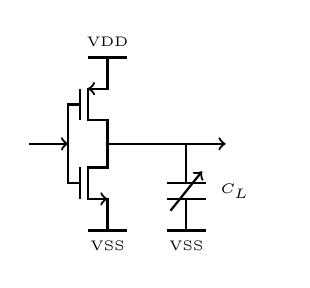
\begin{tikzpicture}
            \draw[thick, ->] (0,0) -- (0.5,0);
            \draw[very thick] (0.75,1.1) -- node[above]{\tiny VDD} (1.25,1.1);
            \draw[very thick] (0.75,-1.1) -- node[below]{\tiny VSS} (1.25,-1.1);
            \draw[thick] (1,1.1) -- (1,0.7) -- (0.75,0.7) -- (0.75,0.3) -- (1,0.3) -- (1,-0.3) -- (0.75,-0.3) -- (0.75,-0.7) -- (1,-0.7) -- (1,-1.1);
            \draw[thick, ->] (1,0.7) -- (0.75,0.7);
            \draw[thick, ->] (0.75,-0.7) -- (1,-0.7);
            \draw[thick] (0.65,0.7) -- (0.65,0.3);
            \draw[thick] (0.65,-0.3) -- (0.65,-0.7);
            \draw[thick] (0.65,0.5) -- (0.5,0.5) -- (0.5, -0.5) -- (0.65,-0.5);
            \draw[thick, ->] (1,0) -- (2.5,0);
            \draw[thick] (2,0) -- (2,-0.5);
            \draw[thick] (1.75,-0.5) -- (2.25,-0.5);
            \draw[thick] (1.75,-0.7) -- (2.25,-0.7);
            \draw[thick] (2,-0.7) -- (2,-1.1);
            \draw[very thick] (2.25,-1.1) -- node[below]{\tiny VSS} (1.75,-1.1);
            \draw[thick, ->] (1.8,-0.85) -- node[inner sep = 12, right]{\tiny $C_L$} (2.2,-0.35);
        \end{tikzpicture}
        \vspace{3.6 mm}
        \captionof{figure}{CMOS ring oscillator stage with varactor load tuning.}
        \label{ring_cap_tuning}
    \end{center}
\end{minipage}
\hspace{0.01\textwidth}
\begin{minipage}{0.4\textwidth}
    \begin{center}
        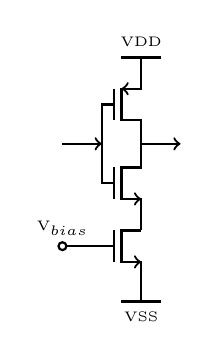
\begin{tikzpicture}
            \draw[thick, ->] (0,0) -- (0.5,0);
            \draw[very thick] (0.75,1.1) -- node[above]{\tiny VDD} (1.25,1.1);
            \draw[very thick] (0.75,-2) -- node[below]{\tiny VSS} (1.25,-2);
            \draw[thick] (1,1.1) -- (1,0.7) -- (0.75,0.7) -- (0.75,0.3) -- (1,0.3) -- (1,-0.3) -- (0.75,-0.3) -- (0.75,-0.7) -- (1,-0.7) -- (1,-1.1);
            \draw[thick, ->] (1,0.7) -- (0.75,0.7);
            \draw[thick, ->] (0.75,-0.7) -- (1,-0.7);
            \draw[thick] (0.65,0.7) -- (0.65,0.3);
            \draw[thick] (0.65,-0.3) -- (0.65,-0.7);
            \draw[thick] (0.65,0.5) -- (0.5,0.5) -- (0.5, -0.5) -- (0.65,-0.5);
            \draw[thick, ->] (1,0) -- (1.5,0);

            \draw[thick] (1,-1.1) -- (0.75,-1.1) -- (0.75,-1.5) -- (1,-1.5) -- (1,-2);
            \draw[thick, ->] (0.75,-1.5) -- (1,-1.5);
            \draw[thick] (0.65,-1.1) -- (0.65,-1.5);
            \draw[thick] (0.65,-1.3) -- (0.05,-1.3);
            \draw[thick] (0,-1.3) circle (0.05) node[above]{\tiny V$_{bias}$};
        \end{tikzpicture}
        \captionof{figure}{CMOS ring oscillator stage with resistive load tuning.}
        \label{ring_res_tuning}
    \end{center}
\end{minipage}

\noindent The LC oscillator is preferred for applications that require low phase noise and high frequency operation. This VCO is based on the
resonator circuit (LC tank) shown in figure \ref{fig:LC_tank_ideal}. The frequency of oscillation of an ideal LC tank is given by \eqref{eq:LC_tank_frequency},
in practice however, there's a need for an active device to compensate for the losses in the circuit and sustain oscillation. This losses, responsible for
dampening the oscillation are primarily caused by the the parasitic series resistance of the inductor.

\begin{equation}
    f_{n} = \frac{1}{2 \pi \sqrt{L C}}
    \label{eq:LC_tank_frequency}
\end{equation}

\begin{minipage}{0.4\textwidth}
    \begin{center}
        \begin{circuitikz}
            \draw[thick] (0,0) to[C = C] (0,4) -- (3,4) to[L = L] (3,0) -- (0,0);
        \end{circuitikz}
        \captionof{figure}{Ideal LC tank circuit.}
        \label{fig:LC_tank_ideal}
    \end{center}
\end{minipage}
\hspace{0.05\textwidth}
\begin{minipage}{0.4\textwidth}
    \begin{center}
        \begin{circuitikz}
            \draw[thick] (0,0) to[C = C] (0,4) -- (3,4) to[L = L] (3,2) to[R = R$_S$] (3,0) -- (0,0);
        \end{circuitikz}
        \captionof{figure}{Real LC tank circuit.}
        \label{LC_tank_real}
    \end{center}
\end{minipage}

\noindent The LC tank of figure \ref{LC_tank_real} can be modeled as a parallel RLC circuit, where the inductor is modeled as an ideal inductor in parallel 
with a resistor ($R_p$) and an ideal capacitor; the equivalent circuit is shown in figure \ref{fig:LC_tank_equivalent}. Equating the transfer functions of both
\ref{LC_tank_real} and \ref{fig:LC_tank_equivalent} yields equation \eqref{eq:LC_tank_equation}, which can be used to compute $R_p$.

\begin{equation}
    -L^2 \omega^2 + R_S R_P + j \omega L R_S = 0
    \label{eq:LC_tank_equation}
\end{equation}

\begin{minipage}{0.4\textwidth}
    \begin{center}
        \begin{circuitikz}
            \draw[thick] (0,0) to[C = C] (0,4) -- (3,4) to[L = L] (3,2) to[R = R$_S$] (3,0) -- (0,0);
        \end{circuitikz}
        \captionof{figure}{Equivalent LC tank circuit.}
        \label{fig:LC_tank_equivalent}
    \end{center}
\end{minipage}
\hspace{0.05\textwidth}
\begin{minipage}{0.4\textwidth}
    \begin{center}
        \begin{circuitikz}
            \draw[thick] 
            node[ground]{} (0,0) to[Tnmos, n = n1, mirror, -o] (0,3)
            (3,0) node[ground]{} to[Tnmos, n = n2, -o] (3,3)
            (n1.G) to[short, -*] (n2.S)
            (n2.G) to[short, -*] (n1.S);
        \end{circuitikz}
        \captionof{figure}{Cross-coupled pair.}
        \label{cross_coupled_pair_schematic}
    \end{center}
\end{minipage}

\noindent The active circuit of figure \ref{cross_coupled_pair_schematic} is known as a cross-coupled pair, it compensates for $R_p$ with a negative resistance. In fact, 
by analyzing the small signal model of the cross-coupled pair the designer can arrive at equation \eqref{eq:cross_coupled_pair_equation}, which allows to solve
for the pair's transconductance ($g_m$). R$_{pair}$ should be chosen $\gg$ R$_p$ so that the former dominates in parallel with the latter (compensating for the 
losses).

\begin{equation}
    R_{pair} = - \frac{2}{g_m}
    \label{eq:cross_coupled_pair_equation}
\end{equation}

\noindent The previous discussion focused on sustaining the oscillations of the LC tank, the control of the frequency is done by changing the capacitance of the tank.
The most common way to do this is by using a varactor, such a device can be implemented with a MOSFET in the triode region and wiring it as shown in figure \ref{fig:varactor_schematic}.
The capacitance of the MOS varactor doesn't change linearly across all of the applied voltage. \ref{MOS_varactor_response} shows the typical response of a MOS varactor in 65 nm, where 
it can be distinguished between three regions: Accumulation region, depletion and inversion. The region of interest is the inversion region, where the capacitance changes 
approximately linearly.

\begin{minipage}{0.4\textwidth}
    \begin{center}
        \begin{circuitikz}
            \draw[thick] (0,0) to[Tnmos, n = n1] (0,1)
            (n1.D) -- (0.5,1.26) -- (0.5, -0.27) -- (n1.S)
            (-0.5,0.5) to[short, -*] (0.5,0.5) node[ground, rotate = 90]{}
            (n1.G) to[short, -o] (-1,0.5) node[above]{$V_{c}$};
        \end{circuitikz}
        \captionof{figure}{MOS varactor.}
        \label{fig:varactor_schematic}
    \end{center}
\end{minipage}
\hspace{0.05\textwidth}
\begin{minipage}{0.4\textwidth}
    \begin{center}
        \begin{tikzpicture}
            \begin{axis}[
                axis lines=left,
                width=\textwidth,
                xlabel={$V_{control}$ (V)},
                ylabel={Capacitance (fF)},
                grid=major
            ]
                \addplot[
                    mark size=0.5pt
                ]
                table[meta=C] {data/MOS_varactor_data.txt};
            \end{axis}
        \end{tikzpicture}
        \captionof{figure}{MOS varactor characteristic.}
        \label{MOS_varactor_response}
    \end{center}
\end{minipage}

\noindent The tuning range can be extended by putting two varactors back to back on their gates. The final circuit of the cross-coupled pair VCO is shown in figure
\ref{fig:cross_coupled_pair_VCO_schematic}.

\begin{center}
    \begin{circuitikz}
        \draw[thick] 
            node[ground]{} (0,0) to[Tnmos, n = n1, mirror] (0,3)
            (3,0) node[ground]{} to[Tnmos, n = n2] (3,3)
            (n1.G) to[short, -*] (n2.S)
            (n2.G) to[short, -*] (n1.S)

            (0,3) to[vC, *-] (1.5,3) to[vC, -*] (3,3)
            (-1,4.5) node[above]{\small $Out_{1}$} to[short, o-] (0,4.5) to[C = C, *-*] (3,4.5) to[short, -o] node[above]{\small $Out_{2}$} (4,4.5)
            (0,6) to[L = L, *-*] (3,6)
            (0,7.5) to[R = R$_P$, *-*] (3,7.5)
            (1.5,3) to[short, *-o] (1.5,3.35) node[above]{$V_c$}
            (3,8.5) -- (3,3)
            (0,8.5) -- (0,3)
            (-1,8.5) -- node[above]{VDD} (4,8.5);
    \end{circuitikz}
    \captionof{figure}{Cross-coupled pair VCO schematic.}
    \label{fig:cross_coupled_pair_VCO_schematic}
\end{center}

\subsubsection{Frequency divider}
The frequency divider is a circuit that takes an input signal and produces an output signal with a frequency that is a fraction of the input frequency.
The most common frequency divider is the flip-flop (fig. \ref{fig:DFF_divider}), which divides the input frequency by two, although there are other types of dividers that can divide by
any integer number. The frequency divider is used in PLLs to reduce the frequency of the input signal to a level that can be processed by the other blocks of the PLL
(to match the frequency of the reference signal).

\begin{minipage}{0.4\textwidth}
    \begin{center}
        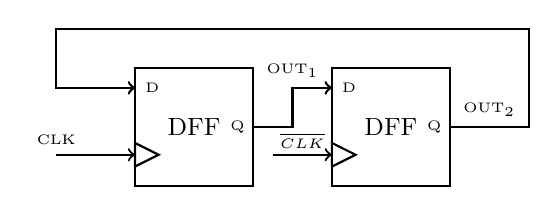
\begin{tikzpicture}
            \draw[thick] (0,0) rectangle (1.5,1.5);
            \draw[thick] (0,0.25) -- (0,0.55) -- (0.3,0.4) -- (0,0.25);
            \draw[->, thick] (-1,0.4) node[anchor=south] {\tiny CLK} -- (0,0.4);
            \draw node at (0.75,0.75) {\small DFF};
            \draw[->, thick] (-1,1.25) -- (0,1.25) node[anchor=west] {\tiny D};
            \draw node at(1.3,0.75) {\tiny Q};
            \draw[->, thick] (1.5,0.75) -- (2,0.75) -- (2,1.25) node[anchor=south] {\tiny OUT$_1$} -- (2.5,1.25);
            \draw[thick] (2.5,0) rectangle (4,1.5);
            \draw[thick] (2.5,0.25) -- (2.5,0.55) -- (2.8,0.4) -- (2.5,0.25);
            \draw[->, thick] (1.75,0.4) -- node[above, inner sep = 2]{\tiny $\overline{CLK}$} (2.5,0.4);
            \draw node at (3.25,0.75) {\small DFF};
            \draw[->, thick] (4,0.75) -- node[above] {\tiny OUT$_2$} (5,0.75) -- (5, 2) -- (-1,2) -- (-1,1.25) -- (0,1.25);
            \draw[->, thick] (2,1.25) -- (2.5,1.25) node[anchor=west] {\tiny D};
            \draw node at(3.8,0.75) {\tiny Q};
        \end{tikzpicture}
        \captionof{figure}{$\%2$ frequency divider using D flip-flops.}
        \label{fig:DFF_divider}
    \end{center}
\end{minipage}
\hspace{0.05\textwidth}
\begin{minipage}{0.4\textwidth}
    \begin{center}
        \begin{circuitikz}
            \draw[thick] (0,0) to[Tnmos, n = n1] (0,1)
            (n1.G) to[short, -o] (-1,0.5) node[left]{\small $V_{bias}$};

            \draw[thick] (-1,2) to[Tnmos, n = n2] (-1,3)
            (n2.G) node[left]{\small $Vin_{1}$}
            (n1.S) node[ground]{}
            (n1.D) -- (-1,1.26) -- (n2.S)
            (n2.D) to[short, -o] node[left]{\small $Vout_{1}$} (-1,3.25) to[R = R1] (-1,5.5);

            \draw[thick] (1,2) to[Tnmos, n = n3, mirror] (1,3)
            (n3.G) node[right]{\small $Vin_{2}$}
            (n3.S) -- (1,1.26) -- (n1.D)
            (n3.D) to[short, -o] node[right]{\small $Vout_{2}$} (1,3.25) to[R = R2, mirror] (1,5.5);

            \draw[very thick] (-2,5.5) -- node[above]{VDD} (2,5.5);

        \end{circuitikz}
        \captionof{figure}{CML frequency divider.}
        \label{fig:CML_divider_schematic}
    \end{center}
\end{minipage}

Although the flip-flop is the most common frequency divider, there are other types of dividers that can be used in PLLs. One of the most relevant is the CML frequency divider (fig. \ref{fig:CML_divider_schematic}),
which is a type of frequency divider that uses current-mode logic (CML) to achieve high speed operation. CML dividers are typically used in high-speed applications, such as
high-speed data communication systems, where the output of the VCO is too high to be processed by any regualr flip-flop. The CML frequency divider is based on the principle of
current steering, where the input signal is used to control the current flowing through a branch of the differential pair.

A CML signal resembles a sinusoidal wave and has a lower harmonic content than a regular square wave, yet its power consumption is higher because of the constant current through the circuit
due to the current source of the differential pair.
\section{Digital phase-locked loop}
One of the main problems of analog PLLs is that they are very sensitive to process, voltage and temperature (PVT) variations, which can cause the PLL to become unstable or to fail to lock.
To address this issue, digital PLLs (DPLLs) have been developed. DPLLs take advantage of the technology scaling (whereas analog PLLs suffer from it) to achieve a better performance
and robustness in modern CMOS processes. To realize a circuit that performs well under this technology nodes it is necessary to avoid the analog domain as much as possible (at least on
the critical path). The fundamental block that allows this task is the time-to-digital converter (TDC).

The general architecture of a digital PLL is shown in figure \ref{fig:DPLL_architecture}. The DPLL consists of a TDC, a digital loop filter (DLF) and a digitally controlled oscillator (DCO).
The basic operation of this three circuits will be explained in the following sections.

\begin{center}
    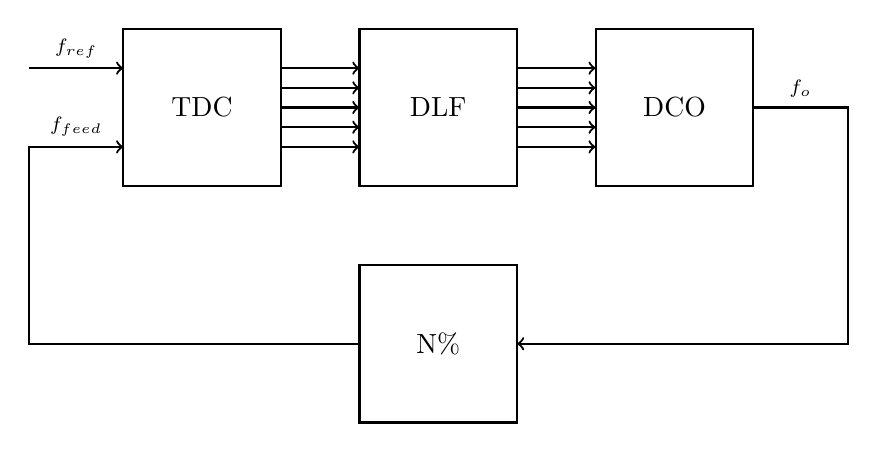
\begin{tikzpicture}
        \draw[thick] (0,0) rectangle (2,2);
        \draw[thick] node at (1,1) {TDC};
        \draw[thick, ->] (-1.2,1.5) -- node[above]{\scriptsize $f_{ref}$} (0,1.5);
        \draw[thick, ->] (2,1.5) -- (3,1.5);
        \draw[thick, ->] (2,1.25) -- (3,1.25);
        \draw[thick, ->] (2,1) -- (3,1);
        \draw[thick, ->] (2,0.75) -- (3,0.75);
        \draw[thick, ->] (2,0.5) -- (3,0.5);
        \draw[thick] (3,0) rectangle (5,2);
        \draw[thick] node at (4,1) {DLF};
        \draw[thick, ->] (5,1.5) -- (6,1.5);
        \draw[thick, ->] (5,1.25) -- (6,1.25);
        \draw[thick, ->] (5,1) -- (6,1);
        \draw[thick, ->] (5,0.75) -- (6,0.75);
        \draw[thick, ->] (5,0.5) -- (6,0.5);
        \draw[thick] (6,0) rectangle (8,2);
        \draw[thick] node at (7,1) {DCO};
        \draw[thick, ->] (8,1) -- node[above]{\scriptsize $f_o$} (9.2,1) -- (9.2,-2) -- (5,-2);
        \draw[thick] (5,-1) rectangle (3,-3);
        \draw[thick] node at (4,-2) {N\%};
        \draw[thick, ->] (3,-2) -- (-1.2,-2) -- (-1.2,0.5) -- node[above]{\scriptsize $f_{feed}$} (0,0.5);

    \end{tikzpicture}
    \captionof{figure}{Digital PLL architecture.}
    \label{fig:DPLL_architecture}
\end{center}

\subsection{Time-to-digital converter}

The TDC substitutes the phase detector of the analog PLL, it measures the time difference ($\Delta_t$) between two signals and converts it into a digital value that is proportional to 
that $\Delta_t$, thus it transforms a signal in the time domain into a signal in the digital domain (avoiding the analog domain entirely). The TDC is a critical block in the DPLL, as 
it determines the resolution and accuracy of the phase measurement. There are several types of TDCs, but the most common one is the delay line TDC, which uses a series of delay elements
to measure the time difference between two signals. A delay line TDC is shown in figure \ref{fig:delay_line_TDC_schematic} and its timing diagram is shown in figure \ref{fig:delay_line_TDC_timing}.

    \begin{center}
        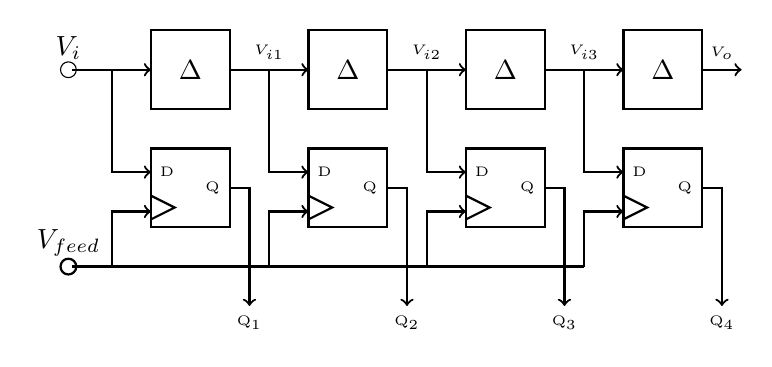
\begin{tikzpicture}
            \draw (-0.05,0.5) node[above]{$V_{i}$} circle (0.1);
            \draw[thick, ->] (0,0.5) -- (1,0.5);
            \draw[thick] (1,0) rectangle (2,1);
            \draw[thick, ->] (0.5, 0.5) -- (0.5,-0.8) -- node[right, inner sep = 10]{\tiny D} (1,-0.8);
            \draw[thick] (1,-1.5) rectangle (2,-0.5);
            \draw[thick] (1,-1.1) -- (1.3,-1.25) -- (1,-1.4);
            \draw[thick, ->] (2,-1) node[left]{\tiny Q} -- (2.25,-1) -- (2.25,-2.5) node[below]{\tiny Q$_1$};
            \draw[thick] node at (1.5,0.5) {$\Delta$};

            \draw[thick, ->] (2,0.5) -- node[above]{\tiny $V_{i1}$} (3,0.5);
            \draw[thick] (3,0) rectangle (4,1);
            \draw[thick, ->] (2.5, 0.5) -- (2.5,-0.8) -- node[right, inner sep = 10]{\tiny D} (3,-0.8);
            \draw[thick] (3,-1.5) rectangle (4,-0.5);
            \draw[thick] (3,-1.1) -- (3.3,-1.25) -- (3,-1.4);
            \draw[thick, ->] (4,-1) node[left]{\tiny Q} -- (4.25,-1) -- (4.25,-2.5) node[below]{\tiny Q$_2$};
            \draw[thick] node at (3.5,0.5) {$\Delta$};

            \draw[thick, ->] (4,0.5) -- node[above]{\tiny $V_{i2}$} (5,0.5);
            \draw[thick] (5,0) rectangle (6,1);
            \draw[thick, ->] (4.5, 0.5) -- (4.5,-0.8) -- node[right, inner sep = 10]{\tiny D} (5,-0.8);
            \draw[thick] (5,-1.5) rectangle (6,-0.5);
            \draw[thick] (5,-1.1) -- (5.3,-1.25) -- (5,-1.4);
            \draw[thick, ->] (6,-1) node[left]{\tiny Q} -- (6.25,-1) -- (6.25,-2.5) node[below]{\tiny Q$_3$};
            \draw[thick] node at (5.5,0.5) {$\Delta$};
            
            \draw[thick, ->] (6,0.5) -- node[above]{\tiny $V_{i3}$} (7,0.5);
            \draw[thick] (7,0) rectangle (8,1);
            \draw[thick, ->] (6.5, 0.5) -- (6.5,-0.8) -- node[right, inner sep = 10]{\tiny D} (7,-0.8);
            \draw[thick] (7,-1.5) rectangle (8,-0.5);
            \draw[thick] (7,-1.1) -- (7.3,-1.25) -- (7,-1.4);
            \draw[thick, ->] (8,-1) node[left]{\tiny Q} -- (8.25,-1) -- (8.25,-2.5) node[below]{\tiny Q$_4$};
            \draw[thick] node at (7.5,0.5) {$\Delta$};
            \draw[thick, ->] (8,0.5) -- node[above]{\tiny $V_o$} (8.5,0.5);

            \draw[thick] (-0.05,-2) node[above]{$V_{feed}$} circle (0.1);
            \draw[thick] (0,-2) -- (6.5,-2);
            \draw[thick, ->] (0.5,-2) -- (0.5,-1.3) -- (1,-1.3);
            \draw[thick, ->] (2.5,-2) -- (2.5,-1.3) -- (3,-1.3);
            \draw[thick, ->] (4.5,-2) -- (4.5,-1.3) -- (5,-1.3);
            \draw[thick, ->] (6.5,-2) -- (6.5,-1.3) -- (7,-1.3);

        \end{tikzpicture}
        \captionof{figure}{Delay line TDC schematic.}
        \label{fig:delay_line_TDC_schematic}
    \end{center}

The TDC of figure \ref{fig:delay_line_TDC_schematic} consists of a series of delay elements ($\Delta$) that are used to measure the time difference between the input signals $V_i$ 
and $V_{feed}$. This delay elements must be identical to each other and have a fixed delay which is the LSB of the TDC. The time difference between the two signals is measured by counting
the number of delay elements that are crossed by the input signal $V_i$ before it reaches the output signal $V_o$ (and both signals are in phase after one complete cycle). The way this is done is by an array of samplers (in this case D flip-flops
but can be any type of sampler) that read the output of each $\Delta$ and hold it until the next clock cycle. Because the outputs of the samplers are sequentially read, the combination
of them represent a digital word in the form of a thermometer code.

The number of delay elements determines the resolution of the TDC and can be calculated as a power of two ($2^n$), thus the number of bits of the TDC with the
waveforms shown in \ref{fig:delay_line_TDC_timing} is given by $2^3 = 8$, after that number of stages the output of the nth delay element would be in phase with the input signal $V_i$.

\begin{center}
    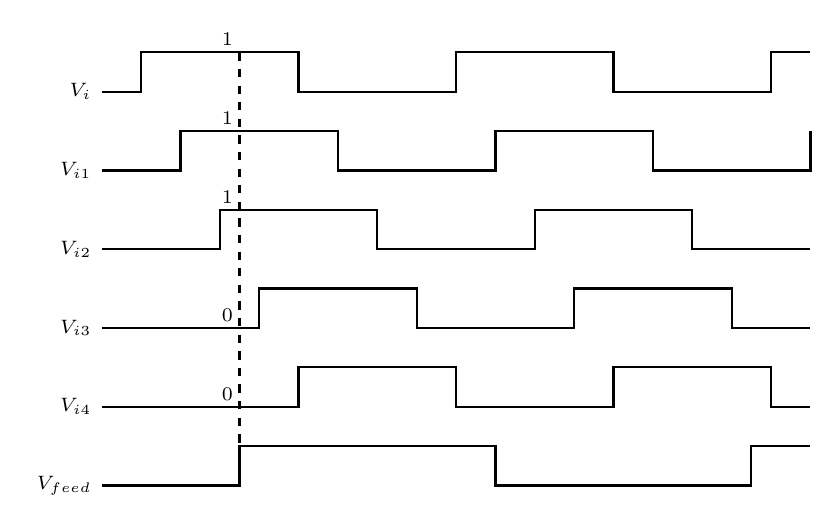
\begin{tikzpicture}
        \draw[thick] (0,0) node[left]{\scriptsize $V_i$} -- (0.5,0) -- (0.5,0.5) -- (2.5,0.5) -- (2.5,0) -- (4.5,0) -- (4.5,0.5) -- (6.5,0.5) -- (6.5,0) -- (8.5,0) -- (8.5,0.5) -- (9,0.5);
        \draw[thick] (0,-1) node[left]{\scriptsize $V_{i1}$} -- (1,-1) -- (1,-0.5) -- (3,-0.5) -- (3,-1) -- (5,-1) -- (5,-0.5) -- (7,-0.5) -- (7,-1) -- (9,-1) -- (9,-0.5);
        \draw[thick] (0,-2) node[left]{\scriptsize $V_{i2}$} -- (1.5,-2) -- (1.5,-1.5) -- (3.5,-1.5) -- (3.5,-2) -- (5.5,-2) -- (5.5,-1.5) -- (7.5,-1.5) -- (7.5,-2) -- (9,-2);
        \draw[thick] (0,-3) node[left]{\scriptsize $V_{i3}$} -- (2,-3) -- (2,-2.5) -- (4,-2.5) -- (4,-3) -- (6,-3) -- (6,-2.5) -- (8,-2.5) -- (8,-3) -- (9,-3);
        \draw[thick] (0,-4) node[left]{\scriptsize $V_{i4}$} -- (2.5,-4) -- (2.5,-3.5) -- (4.5,-3.5) -- (4.5,-4) -- (6.5,-4) -- (6.5,-3.5) -- (8.5,-3.5) -- (8.5,-4) -- (9,-4);
        \draw[thick] (0,-5) node[left]{\scriptsize $V_{feed}$} -- (1.75,-5) -- (1.75,-4.5) -- (5,-4.5) -- (5,-5) -- (8.25,-5) -- (8.25,-4.5) -- (9,-4.5);
        \draw[thick, dashed] (1.75,0.5) node[anchor = south east, inner sep = 2]{\scriptsize 1} -- (1.75,-0.5) node[anchor = south east, inner sep = 2]{\scriptsize 1} -- (1.75,-1.5) node[anchor = south east, inner sep = 2]{\scriptsize 1} -- (1.75,-3) node[anchor = south east, inner sep = 2]{\scriptsize 0} -- (1.75,-4) node[anchor = south east, inner sep = 2]{\scriptsize 0} -- (1.75,-4.5);
    \end{tikzpicture}
    \captionof{figure}{3-bit delay line TDC timing diagram.}
    \label{fig:delay_line_TDC_timing}
\end{center}

It is critically important to design the delay line TDC so that the delays are identical to each other, otherwise the TDC will measure the time difference incorrectly. Furthermore, the
delay elements are usually implemented with a chain of CMOS inverters or differential pairs, both of which are sensitive to process variations, thus the complexity of designing this
otherwise simple circuits. Several techniques have been proposed to address these challenges, such as calibration methods, layout optimization, and the use of delay locked loops (DLLs) to
ensure the delay elements are matched even under PVT variations. The next chapter reviews some of these techniques in detail.

\subsubsection{Delay-locked loop fundamentals}

DLLs are used to generate a stable clock signal that is robust to PVT variations due to negative feedback. The basic operation of a DLL is to compare the phase of an input clock 
signal with a delayed version of itself and adjust the delay of the delayed clock signal until they are in phase. This is done by using a voltage-controlled delay line (VCDL), a phase 
frequency detector (PFD), a charge pump (CP) and a loop filter (LF). Such an architecture is shown in figure \ref{fig:DLL_architecture}.

\begin{center}
    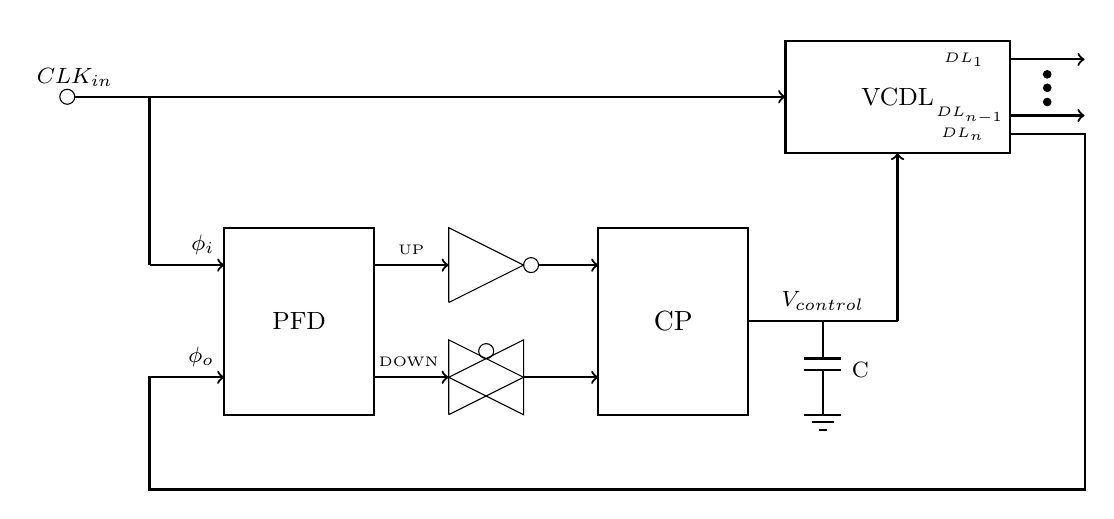
\begin{tikzpicture}[scale=0.95]
            \draw[thick] (0,0) rectangle (2,2.5);   %PFD
            \draw node at (1,1.25) {\small PFD};
            \draw[->, thick] (2,0.5) -- (3,0.5) node[anchor=south east] {\tiny DOWN};
            \draw[->, thick] (2,2) -- (3,2);
            \draw node at (2.5,2.2) {\tiny UP};
            \draw (3,0) -- (3,1) -- (4,0.5) -- (3,0);   %TG
            \draw (3,0.5) -- (4,1) -- (4,0) -- (3,0.5); %NOT
            \draw (3.5,0.85) circle (0.1);
            \draw (3,1.5) -- (3,2.5) -- (4,2) -- (3,1.5);
            \draw (4.1,2) circle (0.1);
            \draw[->, thick] (4.2,2) -- (5,2);
            \draw[->, thick] (4,0.5) -- (5,0.5);
            \draw[thick] (5,2.5) rectangle (7,0);   %CP
            \draw node at (6,1.25) {CP};
            \draw[thick] (7,1.25) -- (9,1.25);  %LF
            \draw[thick] (8,1.25) node[anchor=south] {\footnotesize $V_{control}$} -- (8,0.75);
            \draw[thick] (7.75,0.75) -- (8.25,0.75);
            \draw[thick] (7.75,0.6) -- (8.25,0.6) node[anchor=west] {\footnotesize C};
            \draw[thick] (8,0.6) -- (8,0);
            \draw[thick] (7.75,0) -- (8.25,0);
            \draw[thick] (7.85,-0.1) -- (8.15,-0.1);
            \draw[thick] (7.95,-0.2) -- (8.05,-0.2);
            \draw[->, thick] (9,1.25) -- (9,3.5);
            \draw[thick] (7.5,3.5) rectangle (10.5,5);  %VCDL
            \draw[thick] node at (9,4.25) {\small VCDL};
            \draw[->, thick] (-1,2) -- (-1,4.25) -- (7.5,4.25);
            \draw[->, thick] (-1,2) -- (0,2) node[anchor=south east] {\footnotesize $\phi_i$};
            \draw[thick] (-2,4.25) node[anchor=south] {\footnotesize $CLK_{in}$} -- (-1,4.25);
            \draw (-2.1,4.25) circle (0.1);
            \draw[->, thick] (10.5, 3.75) node[anchor=east, inner sep=9pt] {\tiny $DL_n$} -- (11.5,3.75) -- (11.5,-1) -- (-1,-1) -- (-1, 0.5) -- (0,0.5) node[anchor=south east] {\footnotesize $\phi_o$};
            \draw[->, thick] (10.5, 4) node[anchor=east, inner sep=2pt] {\tiny $DL_{n-1}$} -- (11.5,4);
            \draw[->, thick] (10.5, 4.75) node[anchor=east, inner sep=9pt] {\tiny $DL_{1}$} -- (11.5,4.75);
            \filldraw (11,4.55) circle (0.05);
            \filldraw (11,4.37) circle (0.05);
            \filldraw (11,4.18) circle (0.05);
    \end{tikzpicture}
    \captionof{figure}{DLL architecture.}
    \label{fig:DLL_architecture}
\end{center}

Since the output of the DLL is a delayed version of the input clock signal, it can be used to synchronize the clock signal with the phase of the input clock signal. The delay of the 
VCDL is controlled by the output of the CP, which is in turn controlled by the PFD. The PFD compares the phase of the input clock signal with the delayed version of itself and 
generates an UP or DOWN signal that is used to control the CP. The CP generates a control voltage that is used to adjust the delay of the VCDL until the two clock signals are in phase.
This means that the DLL can be interchangeable with the delay line, thus the TDC can be implemented with a DLL.

\subsection{Digital loop filter}

It has already been mentioned that an analog PLL requires a loop filter to stabilize the feedback loop, the same is true for a DPLL. The digital loop filter (DLF) is used to filter the 
output of the TDC and to generate a control signal that is used to adjust the frequency of the DCO. The DLF is typically implemented as a low-pass filter or a proportional-integral (PI)
controller.

Recalling the first order passive LF of figure \ref{fig:LF_schematic} one can arrive at equation \eqref{eq:LF_transfer_function},where $R_1$ contains the proportional path and 
1/$S \cdot C_1$ contains the integral path.

\begin{equation}
    H(s) = R_1 + \frac{1}{S \cdot C_1}
    \label{eq:LF_transfer_function}
\end{equation}

\begin{minipage}
{0.4\textwidth}
    \begin{center}
        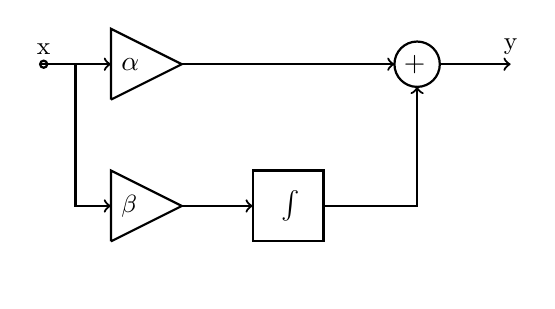
\begin{tikzpicture}[scale = 0.9]
            \draw node[above] at (0.05,0) {\small x};
            \draw[thick] (0.05,0) circle (0.05);
            \draw[thick, ->] (0,0) -- (1,0) node[right]{$\alpha$};
            \draw[thick] (1,-0.5) -- (1,0.5) -- (2,0) -- (1,-0.5);
            \draw[thick, ->] (2,0) -- (5,0) node[right, inner sep = 3]{$+$};
            \draw[thick] (5.32,0) circle (0.32);
            \draw[thick, ->] (5.64,0) -- (6.64,0) node[above]{\small y};
            \draw[thick, ->] (0.5,0) -- (0.5,-2) -- (1,-2) node[right]{\small $\beta$};
            \draw[thick] (1,-2.5) -- (1,-1.5) -- (2,-2) -- (1,-2.5);
            \draw[thick, ->] (2,-2) -- (3,-2) node[right, inner sep = 10]{\small $\int$};
            \draw[thick] (3,-2.5) rectangle (4,-1.5);
            \draw[thick, ->] (4,-2) -- (5.32,-2) -- (5.32,-0.32);

            \draw[color=white] (0,-2.75) rectangle (6.64,-3.05);
        \end{tikzpicture}
        \captionof{figure}{Conceptual filter using a proportional and an integral path.}
        \label{fig:LF_conceptual_topology}
    \end{center}
\end{minipage}
\hspace{0.05\textwidth}
\begin{minipage}{0.4\textwidth}
    \begin{center}
        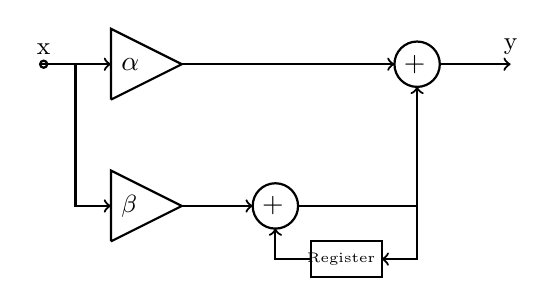
\begin{tikzpicture}[scale = 0.9]
            \draw node[above] at (0.05,0) {\small x};
            \draw[thick] (0.05,0) circle (0.05);
            \draw[thick, ->] (0,0) -- (1,0) node[right]{$\alpha$};
            \draw[thick] (1,-0.5) -- (1,0.5) -- (2,0) -- (1,-0.5);
            \draw[thick, ->] (2,0) -- (5,0) node[right, inner sep = 3]{$+$};
            \draw[thick] (5.32,0) circle (0.32);
            \draw[thick, ->] (5.64,0) -- (6.64,0) node[above]{\small y};
            \draw[thick, ->] (0.5,0) -- (0.5,-2) -- (1,-2) node[right]{\small $\beta$};
            \draw[thick] (1,-2.5) -- (1,-1.5) -- (2,-2) -- (1,-2.5);
            \draw[thick, ->] (2,-2) -- (3,-2) node[right, inner sep = 3]{$+$};
            \draw[thick] (3.32,-2) circle (0.32);
            \draw[thick, ->] (3.64,-2) -- (5.32,-2) -- (5.32,-0.32);
            \draw[thick, ->] (5.32,-2) -- (5.32,-2.75) -- (4.82,-2.75) node[left, inner sep = 2]{\tiny Register};
            \draw[thick] (4.82,-3) rectangle (3.82,-2.5);
            \draw[thick, ->] (3.82,-2.75) -- (3.32,-2.75) -- (3.32,-2.32);
        \end{tikzpicture}
        \captionof{figure}{DLF implementation using an adder and a register.}
        \label{fig:DLF_implementation}
    \end{center}
\end{minipage}

Knowing the analog transfer function of the LF, a conceptual topology similar to that of figure \ref{fig:LF_conceptual_topology} could be proposed, where $y = \alpha + \beta \int_{}^{} x \,dx$
for continuous-time quantities. To arrive at a digital counterpart, one could change x to D$_{in}$ and y to D$_{out}$, rewrite this equation as the discrete-time expression
\eqref{eq:conceptual_equation}, and take the Z transform of both sides to obtain the transfer function of the DLF \eqref{eq_DLF_transfer_function}, noting that a discrete-time integrator
is represented by $1/(1 - z^{-1})$ [Razavi PLL book reference].

\begin{equation}
    D_{out}(k) = \alpha + \beta \sum_{k=0}^{\infty} D_{in}[k]
    \label{eq:conceptual_equation}
\end{equation}

\begin{equation}
    H(z) = \frac{D_{out}}{D_{in}}(z) = \alpha + \frac{\beta}{1 - z^{-1}}
    \label{eq_DLF_transfer_function}
\end{equation}

Depicted in figure \ref{fig:DLF_implementation} is an implementation of the DLF that realizes the discrete-time integrator as an accumulator consisting of an adder and a register. The
clock of such register is typically the same as the PLL reference.

\subsection{Digitally controlled oscillator}

Having already discussed the VCO fundamentals and a couple of implementations, the digitally controlled oscillator (DCO) can be viewed as a VCO that is controlled by a digital word instead
of an analog voltage. Taking a look back at the VCO schematic of figure \ref{fig:cross_coupled_pair_VCO_schematic} it can be observed that the frequency is controlled by the bias
voltage $V_c$ at the gate of both MOSFET varactors. If the varactors are replaced by either a binary weighted capacitor array or current steering DAC, then the frequency of the circuit can
be controlled digitally.

\begin{center}
    \begin{circuitikz}
        \draw[thick] 
            (0,-1.5) node[ground]{} (0,-1.5) to[Tnmos, n = n1, mirror] (0,1.5)
            (3,-1.5) node[ground]{} to[Tnmos, n = n2] (3,1.5)
            (n1.G) to[short, -*] (n2.S)
            (n2.G) to[short, -*] (n1.S)

            (-1,4.5) node[above]{\small $Out_{1}$} to[short, o-] (0,4.5) to[C = C$_u$, *-] (1,4.5) to[switch = D$_0$] (2,4.5) to[C = C$_u$, -*] (3,4.5) to[short, -o] node[above]{\small $Out_{2}$} (4,4.5)
            (0,3) to[C = 2 C$_u$, *-] (1,3) to[switch = D$_1$] (2,3) to[C = 2 C$_u$, -*] (3,3)
            (0,1.5) to[C = 4 C$_u$, *-] (1,1.5) to[switch = D$_2$] (2,1.5) to[C = 4 C$_u$, -*] (3,1.5)
            (0,6) to[L = L, *-*] (3,6)
            (0,7.5) to[R = R$_P$, *-*] (3,7.5)

            (3,8.5) -- (3,1.5)
            (0,8.5) -- (0,1.5)
            (-1,8.5) -- node[above]{VDD} (4,8.5);
    \end{circuitikz}
    \captionof{figure}{Cross-coupled DCO implementation with binary weighted capacitive array.}
    \label{fig:DCO_schematic}
\end{center}

Figure \ref{fig:DCO_schematic} shows a cross-coupled DCO realization that makes use of a binary weighted capacitor array as the control mechanism. This binary weighted branches
are controlled by switches that must be transmission gates (TG) because of the differential nature of the circuit. When the switches are closed, the capacitance of the
branches is added to the total capacitance of the circuit, thus reducing the frequency of oscillation. It is desirable that the reverse occurs, so the digital word is
typically inverted before being applied to the switches, that way if the digital word rises from one cycle to the next the frequency of oscillation will also rise.

It is necessary to pay attention to the design of this capacitive array because the parasitic capacitance of the switches and the interconnects can significantly alter the 
desired frequency step of the DCO, another factor to take into account is the mismatch between the capacitors, which can cause the frequency steps to be uneven. To mitigate these issues
minimum capacitor values should be avoided if possible.